\documentclass[a4paper,12pt,onecolumn]{article}

\usepackage[utf8]{inputenc}
\usepackage[english]{babel}
\usepackage{amssymb,amsmath,amsthm,array,epsfig,a4,verbatim,pstricks,url,subfig,
hyperref}

\newenvironment{keywords}{{\upshape\bfseries Key words. }\ignorespaces}{}

\newtheorem{thm}{Theorem}
\newtheorem{lem}{Lemma}

\newcommand{\R}{{\mathbb R}}
\newcommand{\spa}{\operatorname{span}}
\newcommand{\vol}{\mathcal{L}^d}
\newcommand{\dH}[1]{\;{\rm d}{\cal H}^{#1}} % Hausdorff measure
\newcommand{\dL}[1]{\;{\rm d}{\cal L}^{#1}} % Lebesgue measure
\newcommand{\bigchi}{\ensuremath{\mathrm{\mathcal{X}}}}
\newcommand{\charfcn}[1]{\bigchi_{#1}} % characteristic function
\newcommand{\Vh}{\underline{V}(\Gamma^m)}
\newcommand{\Wh}{W(\Gamma^m)}
\newcommand{\Vht}{\underline{V}(\Gamma^h(t))}
\newcommand{\Wht}{W(\Gamma^h(t))}
\newcommand{\uspace}{\mathbb{U}}
\newcommand{\pspace}{\mathbb{P}}
\newcommand{\kspace}{\mathbb{K}}
\newcommand{\xspace}{\mathbb{X}}
\newcommand{\sigmaO}{o}
\newcommand{\nabs}{\nabla_{\!s}}
\newcommand{\Id}{I\!d}
\newcommand{\id}{\rm id}
\newcommand{\ddt}{\frac{\rm d}{{\rm d}t}}
\newcommand{\NbulkT}{\vec{N}_{\Gamma,\Omega}^T}
\newcommand{\Nbulk}{\vec{N}_{\Gamma,\Omega}}
\newcommand{\errorXx}{\|\Gamma^h - \Gamma\|_{L^\infty}}
\newcommand{\LerrorUu}[1]{\|\vec U - I^h_{#1}\,\vec u\|_{L^2(\Omega_T)}}
\newcommand{\errorUu}[1]{\|\vec U - I^h_{#1}\,\vec u\|_{L^\infty}}
\newcommand{\errorPp}[1]{\|P - I^h_{#1}\,p\|_{L^\infty}}
\newcommand{\LerrorPp}{\|P - p\|_{L^2(\Omega_T)}}
\newcommand{\unitn}{\vec{\rm n}}
\newcommand{\mat}[1]{\underline{\underline{#1}}\rule{0pt}{0pt}}

\renewcommand{\theequation}{\arabic{section}.\arabic{equation}}

\begin{document}

\captionsetup[subfigure]{labelformat=empty} % remove label subplot
\newcolumntype{H}{>{\setbox0=\hbox\bgroup}c<{\egroup}@{}} % hide table column

\begin{abstract}
We propose a novel fitted finite element method for two-phase Stokes flow
problems that uses piecewise linear finite elements to approximate the
moving interface. The method can be shown to be unconditionally stable.
Moreover, spherical stationary solutions are captured exactly by the numerical
approximation. In addition, the meshes describing the discrete interface in
general do not deteriorate in time, which means that in numerical simulations a
smoothing or a remeshing of the interface mesh is not necessary. We present
several numerical experiments for our numerical method, which demonstrate the
accuracy and robustness of the proposed algorithm.
\end{abstract}

\begin{keywords}
viscous incompressible two-phase flow, Stokes equations, free boundary problem,
surface tension, finite elements, front tracking
\end{keywords}

\section{Introduction}\label{sec:introduction}
Fluid flow problems with a moving interface are encountered in many
applications in physics, engineering and biophysics. Developing robust and
efficient numerical methods for these flows is an important problem and has
attracted tremendous interest over the last decade. Apart from the usual
difficulties arising from the numerical computation of the fluid flow in the
bulk, the acurate approximation of the moving free interface, as well as a
suitable description of the conditions that need to hold on the interface, pose
serious challenges. Of particular importance is the precise inclusion of surface
tension terms, and the correct handling of discontinuity jumps in material
properties and pressure at the interface, in order to suppress spurious
velocities, which are also called parasitic currents.

In this paper we propose a novel finite element approximation for
incompressible two-phase Stokes flow that naturally avoids spurious velocities.
Our scheme is based on the numerical method introduced in \cite{spurious}, and
so uses piecewise linear parametric finite elements to describe the moving
discrete interface. In contrast to \cite{spurious}, where the interface and the
bulk mesh were totally independent, here we pursue the fitted approach. That
means that the interface discretization is always fitted to the bulk mesh, i.e.\
the discrete interface is made up of edges/faces of element belonging to the
bulk mesh. An advantage of our method is that the discontinuity jumps in
material properties and in the pressure are captured naturally. In particular,
we do not need to employ an XFEM-type extension of standard bulk pressure
spaces.
Surface tension forces are discretized with the help of a variational
approximation of curvature that was first proposed in \cite{triplej,gflows3d}.
Combining this was an implicit treatment of the surface tension forces yields an
unconditionally stable scheme. Interestingly, the formulation of curvature from
\cite{triplej} leads to a tangential motion of vertices in practice, which
guarantees equidistribution in 2d and good meshes in 3d. Overall, our proposed
method has the following properties.
\begin{itemize}
\item The fully discrete scheme is unconditionally stable in the sense that the
total surface energy is monotonically decreasing independent of the chosen time
step size.
\item In the absence of outer forces, any discrete solution with a stationary
interface must have zero velocity globally, i.e.\ we can prove that there are no
stationary solutions with spurious velocities. Similarly, discrete stationary
solutions for spherical interface are attained for our scheme.
\item For the semidiscrete continuous-in-time variant of the scheme the volume
of the two phases is conserved. The fully discrete scheme maintains the enclosed
volumes well.
\item Thanks to the fitted nature of the finite element method, the pressure
jumps at the interface are captured accurately for standard pressure finite
element spaces without the need for XFEM extensions.
\item The surface tension effects are included with the help of a variational
treatment of curvature based on the Laplace--Beltrami operator.
\item The surface mesh quality is maintained. In particular, for the
semidiscrete scheme an equidistribution property can be shown in 2d.
\item The fully discrete scheme uses an implicit approximation of curvature
that leads to a linear system of equations to be solved at each time step.
\end{itemize}

Let us briefly discuss alternative approaches to the numerical approximation of
two-phase flow problems. In this paper we use a direct description of the
interface using a parameterization of the unknown interface. In such direct
approaches, which are often called front-tracking methods, the interface is
either triangulated or presented by a connected set of particles. The discrete
interface is advected with the help of the bulk fluid velocities, and quantities
on the interface need to be suitably coupled to the bulk equations. We refer
e.g.\ to
\cite{UnverdiT92,Bansch01,Tryggvason_etal01,GanesanMT07,GanesanT08,spurious}
for further details, and to \cite{LevequeL97,Peskin02} for the related immersed
boundary method. Another class of approaches is based on interface capturing
methods using an indicator function to describe the interface. The volume of
fluid (VOF) method and the level set  method fall into this category. In the
former, the characteristic function of one of the phases is approximated
numerically, see e.g.\ \cite{HirtN81,RenardyR02,Popinet09}; whereas in the
latter, the interface is given as the level set of a function, which has to be
determined, see e.g.\ \cite{SussmanSO94,Sethian99,OsherF03,GrossR07}. In phase
field methods the interface is assumed to have a small, but positive, thickness
and an additional parabolic equation, defined in the whole domain, has to be
solved in these so-called diffuse interface models. We refer to
\cite{HohenbergH77,AndersonMW98,LowengrubT98,Feng06,KaySW08,AbelsGG12,GrunK14}
for details.

The remainder of this paper is organized as follows. In
Section~\ref{sec:problem} we present the mathematical model and the weak
formulation on which our finite element approximation is going to be based. Our
numerical method is presented in Section~\ref{sec:fem}, together with proofs for
its main properties. In addition, we describe how the arising linear systems of
equations are solved in practice, and we give details on our mesh generation and
smoothing procedures. Finally, in Section~\ref{sec:numerical_results} we present
several numerical simulations in 2d and 3d.

\begin{figure}[htbp]
  \centering
  \subfloat[Stationary bubble problem]{\includegraphics[width=.45\textwidth]
  {figures/mesh_uniform.ps}}\quad
  \subfloat[Expanding bubble problem]{\includegraphics[width=.45\textwidth]
  {figures/mesh_hole_uniform.ps}}\\
  \caption{Initial fitted uniform 2D meshes with 32 interface elements.}
  \label{fig:meshes_uniform}
\end{figure}

\begin{figure}[htbp]
  \centering
  \subfloat[Stationary bubble problem]{\includegraphics[width=.45\textwidth]
  {figures/mesh_adaptive.ps}}\quad
  \subfloat[Expanding bubble problem]{\includegraphics[width=.45\textwidth]
  {figures/mesh_hole_adaptive.ps}}\\
  \caption{Initial fitted adaptive 2D meshes with 64 interface elements.}
  \label{fig:meshes_adaptive}
\end{figure}

\section{Schur complement approach}\label{sec:shur}

\textcolor{magenta}{TODO : why I am calculating twice the factorization of
(\ref{eq:Xi}) in my code??}

For the the solution of (\ref{eq:lin}) we use a Schur complement approach that
eliminates $(\kappa^{m+1}, \delta \vec X^{m+1})$ from (\ref{eq:lin}), and then
use an iterative solver for the remaining system in $(\vec U^{m+1}, P^{m+1})$.
This approach has the advantage that for the reduced system well-known solution
methods for finite element discretizations for the standard Stokes equations may
be employed. The desired Schur complement approach for eliminating
$(\kappa^{m+1},\delta \vec X^{m+1})$ from (\ref{eq:lin}) can be obtained as
follows. Let
\begin{equation} \label{eq:Xi}
\Xi_\Gamma:= \begin{pmatrix}
 0 & - \frac1{\tau_m}\,\vec{N}_\Gamma^T \\
\vec{N}_\Gamma & \vec{A}_\Gamma
\end{pmatrix} \,.
\end{equation}
Then (\ref{eq:lin}) can be reduced to
\begin{subequations}
\begin{equation} \label{eq:SchurkX}
\begin{pmatrix}
\vec B_\Omega + \gamma\,(\Nbulk \ 0)\,\Xi_\Gamma^{-1}\,
\binom{\NbulkT}{0} & \vec C_\Omega \\
\vec C_\Omega^T & 0
\end{pmatrix}
\begin{pmatrix}
\vec U^{m+1} \\ P^{m+1}
\end{pmatrix}
= \begin{pmatrix}
\vec g
-\gamma\,(\Nbulk \ 0)\, \Xi_\Gamma^{-1}\,
\binom{0}{\vec{A}_\Gamma\,\vec{X}^{m}} \\
0
\end{pmatrix}
\end{equation}
and
\begin{equation}
\binom{\kappa^{m+1}}{\delta\vec{X}^{m+1}} = \Xi_\Gamma^{-1}\,
\binom{-\NbulkT\,\vec U^{m+1}}{-\vec{A}_\Gamma\,\vec{X}^{m}}\,.
\label{eq:SchurkXb}
\end{equation}
\end{subequations}

We notice that when $\gamma = 0$ the linear system (\ref{eq:SchurkX}) becomes
\begin{equation} \label{eq:stokes_system}
\begin{pmatrix}
\vec B_\Omega & \vec C_\Omega \\
\vec C_\Omega^T & 0
\end{pmatrix}
\begin{pmatrix}
\vec U^{m+1} \\ P^{m+1}
\end{pmatrix}
= \begin{pmatrix}
\vec g \\
0
\end{pmatrix}\,,
\end{equation}
which for $\mu_+=\mu_-$ corresponds to a discretization of the one--phase
Stokes problem. This system is well known and a classical way to solve it is to
use a preconditioned GMRES iteration with the preconditioner
\begin{equation} \label{eq:ESW}
\mathcal{P} = \begin{pmatrix}
\vec{\mathcal{P}}_{\vec B} & \vec C_\Omega \\
0 & -\mathcal{P}_S
\end{pmatrix}\,,
\end{equation}
where $\vec{\mathcal{P}}_{\vec B}$ is some preconditioner for the matrix $\vec
B_\Omega$, and $\mathcal{P}_S$ acts as a preconditioner for the Schur complement
operator $S=\vec C^T_\Omega \,\vec B_\Omega^{-1}\,\vec C_\Omega$.

An application of the preconditioner (\ref{eq:ESW}) amounts to solving the
equations
\begin{equation*}
\begin{pmatrix}
\vec{\mathcal{P}}_{\vec B} & \vec C_\Omega \\
0 & -\mathcal{P}_S
\end{pmatrix}
\begin{pmatrix} \vec U \\ P \end{pmatrix}
= \begin{pmatrix} \vec v \\ q \end{pmatrix}
\iff
\mathcal{P}_S\,P = -q\,,\quad \vec{\mathcal{P}}_{\vec B}\,\vec U = \vec v -
\vec C_\Omega\,P\,.
\end{equation*}

Therefore, we solve (\ref{eq:SchurkX}), which is a slight modification of
(\ref{eq:stokes_system}), with a preconditioned GMRES iteration, and we choose
$\vec B_\Omega$  for $\vec{\mathcal{P}}_{\vec B}$ and the weighted mass matrix $
M_\mu$
\begin{equation*}
[M_\mu]_{nq} = \left((\mu^m)^{-1}\,\phi_q^{\pspace^m},
\phi_n^{\pspace^m}\right) \qquad n,q = 1 ,\ldots, K_\pspace^m\,
\end{equation*}
for $\mathcal{P}_S$.
At each iteration of the GMRES, the matrix (\ref{eq:Xi}) needs to be
"inverted`` (more precisely the linear system associated to that matrix needs to
be solved), therefore we use the UMFPACK, see
\cite{UMFPACK,suitesparse-web-page}, direct linear solver to reuse the
factorization.

In our numerical simulations, we always set the GMRES tolerance to $10^{-12}$
and the restart value to 1000.

When we use use the space (P1+P0) for the pressure, (\ref{eq:SchurkX}) becomes
\begin{subequations}
\begin{equation} \label{eq:SchurkXP1P0}
\begin{pmatrix}
\vec B_\Omega + \gamma\,(\Nbulk \ 0)\,\Xi_\Gamma^{-1}\,\binom{\NbulkT}{0} &
\vec C_{\Omega,1} & \vec C_{\Omega,0} \\
\vec C^T_{\Omega,1} & 0 & 0 \\
\vec C^T_{\Omega,0} & 0 & 0 \\
\end{pmatrix}
\begin{pmatrix}
\vec U^{m+1} \\
P^{m+1}_1 \\
P^{m+1}_0
\end{pmatrix}
= \begin{pmatrix}
\vec g-\gamma\,(\Nbulk \ 0)\,
\Xi_\Gamma^{-1}\,\binom{0}{\vec{A}_\Gamma\,\vec{X}^{m}} \\
0 \\
0
\end{pmatrix}
\end{equation}
\end{subequations}
and an application of the preconditioner amounts to solving the equations
\begin{equation*}
\begin{pmatrix}
\vec{\mathcal{P}}_{\vec B} & \vec C_{\Omega,1} & \vec C_{\Omega,0} \\
0 & -\mathcal{P}_{S,1} & 0 \\
0 & 0 &-\mathcal{P}_{S,0}
\end{pmatrix}
\begin{pmatrix}
\vec U \\
P_1 \\
P_0
\end{pmatrix}
=
\begin{pmatrix}
\vec v \\
q \\
p
\end{pmatrix}
\end{equation*}
which is
\begin{equation*}
\mathcal{P}_{S,1}\,P_1 = -q\,,\quad \mathcal{P}_{S,0}\,P_0 = -p\,,\quad \vec{\mathcal{P}}_{\vec B}\,\vec U = \vec v - \vec C_{\Omega,1}\,P_1 - \vec C_{\Omega,0}\,P_0\,.
\end{equation*}

\section{Preservation of mesh quality}

Depending on the nature of problem, the bulk elements around the interface may
have a quick distortion and may overlap leading to a drastic decrease of the
accuracy of the scheme. To prevent this, it is necessary to keep a good mesh
quality throughout all the simulation. We adopt and combine two different
methods to accomplish the preservation of the mesh quality, namely mesh
smoothing and remeshing.

\subsection{Mesh smoothing} \label{subsec:smoothing}

\textcolor{magenta}{TODO : add proper explanation, ALE in general seems a way
to rewrite an equation respect to a manifold}

We use a deforming grid technique to smooth the bulk mesh called Arbitrary
Lagrangian Eulerian (ALE) approach, see \cite{GanesanPhd} for more details. In
this approach the interfaces move with the fluid while the inner mesh points can
be displaced in an arbitrarily prescribed way. This avoids the quick distortion
of meshes and remeshing almost. More precisely the interface points $\vec x \in
\Gamma(t)$ are advected with the bulk velocity
\begin{equation}\label{eq:smoothing_ALE}
\vec{\mathcal{V}}\,.\,\vec\nu = \vec u\,.\,\vec \nu\quad \mbox{on }\Gamma(t)
\end{equation}
while the inner points can be moved arbitrarily to preserve the mesh quality.
Several techniques are proposed in the literature for the inner points
displacements. It is worth to notice that (\ref{eq:smoothing_ALE}) holds only
for the interface in the ALE approach. When it holds on the entire domains
$\Omega_{\pm}(t)$ it is called Lagrangian approach and also the inner mesh
points move with the prescribed velocity.

We use the so called linear elastic solid technique to prescribe the inner
points displacement with respect to the interface displacement. The problem to
solve is: find a map $\vec \psi$ such that
\begin{align}
 \nabla\,.\mat S(\vec \psi) &= 0 && \mbox{in }\Omega_{\pm}(t)\\
 \vec \psi &= \delta \vec X && \mbox{on } \Gamma(t)
\end{align}
where
\begin{equation} \label{eq:elasticity_tensor}
\mat S(\vec \psi) = \lambda_1 \,(\nabla\,.\vec\psi)\mat\id + 2\,\lambda_2\,
\mat D(\vec\psi).
\end{equation}
We stress the fact that the unknown $\vec\psi$ is the displacement which all
the mesh bulk points are subjected to after the smoothing respect the actual
mesh. As condition, we are imposing that the bulk mesh points which lay on the
interface, (remember that we are using a fitted approach), remains fixed after
the smoothing.

The weak formulation is: find $\vec\psi\in \mathbb{M}= H^1(\Omega, \R^d)$ such that
\begin{equation}
\big(\,\mat D(\vec\psi)\,,\,\mat D (\vec \phi)\,\big)+ C_s\,\big(\,
\nabla\,.\,\vec \psi\,,\,\nabla\,.\,\vec\phi\,\big)\, =\, 0\quad \forall \vec
\phi \in\mathbb{M}
\end{equation}
with free-slip condition on $\partial\Omega$ and with smoothing coefficient
$C_s=\frac{\lambda_1}{\lambda_2}>0$.

The algebraic system is solved with UMFPACK.

\subsection{Remeshing} \label{subsec:remeshing}

After the smoothing process, we check the bulk mesh quality computing the
volume ratio of the elements. More precisely, if the following inequality is
satisfied
\begin{equation}\label{eq:remesh_criteria}
\frac{\max_{\sigmaO\in {\cal
T}^m}(\mathcal{H}^{d}(\sigmaO))}{\min_{\sigmaO\in\mathcal
{T}^m}(\mathcal{H}^{d}(\sigmaO))}<C_r,
\end{equation}
the mesh quality is good enough to continue the simulation. We call $C_r>0$
remeshing coefficient.

When (\ref{eq:remesh_criteria}) is not satisfied, the bulk mesh is too deformed
and, in order to preserve the mesh quality, we rebuild the bulk mesh from
scratch keeping the interface mesh and the bulk boundary fixed. Obviously, when
$C_r\leq 1$ a remeshing is always called. We stress the fact that, like in the
mesh smoothing, the interface needs to remain fixed.

\section{Numerical results} \label{sec:numerical_results}

The simplest test is the so called stationary bubble. In this experiment we
solve the trivial true solution of a stationary $d-1$--sphere. In particular,
$\Gamma(t) := \{ \vec z \in \R^d : |\vec z| = r(t)\}$, where
\begin{subequations}
\begin{equation} \label{eq:radialr}
r(t) = r(0)\,,
\end{equation}
together with
\begin{equation} \label{eq:radialup}
\vec u(\vec z, t) = \vec 0 \,,\quad p(\vec z, t) =
\lambda(t)\left[\charfcn{\Omega_-(0)}
-\frac{\mathcal{L}^d(\Omega_-(0))}{\mathcal{L}^d(\Omega)} \right] ,
\end{equation}
\end{subequations}
where $\lambda(t) = \lambda(0) = \gamma\,(d-1)\,[r(0)]^{-1}$, is an exact
solution to the problem (\ref{eq:full_momentum}--g).

A nontrivial divergence free and radially symmetric solution $\vec u$ can be
constructed on a domain that does not contain the origin. To this end, consider
e.g.\ $\Omega = (-H,H)^d \setminus [-H_0, H_0]^d$, with $0 < H_0 < H$. Then
$\Gamma(t) := \{ \vec z \in \R^d : |\vec z| = r(t)\}$, where
\begin{subequations}
\begin{equation} \label{eq:radialr2}
r(t) = ([r(0)]^d + \alpha\,t\,d)^\frac1d \,,
\end{equation}
together with
\begin{equation} \label{eq:radialup2}
\vec u(\vec z, t) = \alpha\,|\vec z|^{-d}\,\vec z \,, \quad p(\vec z, t) =
\lambda(t)\left[ \charfcn{\Omega_-(t)} -
\frac{\mathcal{L}^d(\Omega_-(t))}{\mathcal{L}^d(\Omega)}\right],
\end{equation}
\end{subequations}
where $\lambda(t) = \gamma\,(d-1)\,[r(t)]^{-1} + 2\,\alpha\,(d-1)\,(\mu_+ -
\mu_-)\,[r(t)]^{-d}$, is an exact solution to the problem
(\ref{eq:full_momentum}--g) with the homogeneous right hand side in
(\ref{eq:full_initial_velocity}) replaced by $\vec g$, where $\vec g(\vec z) =
\alpha\,|\vec z|^{-d}\,\vec z$. We call this experiment expanding bubble.

In the following, we fix, as initial interface, the surface $\Gamma(0) = \{
\vec z \in \R^d : |\vec z| = \frac12 \}$ and we use uniform time steps
$\tau_m=\tau$, $m=0,\ldots, M-1$.

Finally, we define the errors
\begin{equation} \label{eq:errorXx}
\errorXx := \max_{m=1,\ldots, M} \|\Gamma^m - \Gamma(t_m)\|_{L^\infty}\,,
\end{equation}
where $\|\Gamma^m - \Gamma(t_m)\|_{L^\infty} :=
\max_{k=1,\ldots, K_\Gamma} {\rm dist}( \vec{q}^m_k, \Gamma(t_m))$,
\begin{equation*}
\errorUu2 := \max_{m=1,\ldots, M}\|U^m - \vec
I^m_2\,u(\cdot,t_m)\|_{L^\infty(\Omega)}\,,
\end{equation*}
and
\begin{equation*}
\LerrorPp := \left[\tau\,\sum_{m=1}^M \|P^m - p(\cdot,t_m)\|_{L^2(\Omega)}^2
\right]^\frac12\,,
\end{equation*}
where for the $L^2$--norms over $\Omega$ we employ a quadrature rule of degree
$k$, with $k=13$ in 2d and $k=10$ in 3d.

\subsection{Numerical results in 2d} \label{subsec:numerical_results_2d}

For the stationary bubble test we use the domain $\Omega = (-1,1)^2$ and we
choose, for the true solution (\ref{eq:radialr},b), the parameters
\begin{equation*}
\mu = \gamma = 1\,.
\end{equation*}
Therefore, the true solution reduces to $r(t) = \frac{1}{2}$, $\vec u(\cdot, t)
= \vec 0$ and $p(t) = 2\,\charfcn{\Omega_-(0)} - \frac{\pi}{8}$ for all $t \geq
0$.

In Table~\ref{tab:bubble2Delementsuniform} it is reported the characteristic
length $c_l$, used to create the mesh for the stationary bubble problem, the
corresponding number of interface elements $K_\Gamma$ generated, the
corresponding number of bulk elements $K_\Omega$ generated and the time step
$\tau$ used. All these meshes are uniform so the same characteristic length is
used both for the interface and for the boundary.

The characteristic length prescribes the size of the mesh elements. For
example, a segment of length $L$, which defines an edge of the domain boundary,
delimited by two points of characteristic length $c_l$ will be subdivided into
several segments of lengths $\frac{L}{c_l}$ during the mesh generation.
Therefore, smaller is the characteristic length, finer is the resulting mesh.
\begin{table*}
 \center
\begin{tabular}{llll}
\hline
$c_l$ & $K_\Gamma$ & $K_\Omega$ & $\tau$ \\
\hline
0.25 & 16 & 224 & $10^{-2}$ \\
0.1 & 32 & 1076 & $10^{-2}$\\
0.05 & 64 & 4240 & $10^{-2}$\\
0.025 & 128 & 17194 & $10^{-2}$ \\
\hline
\end{tabular}
\caption{Number of interface elements ($K_\Gamma$), number of bulk elements
($K_\Omega$) and time step ($\tau$) for a certain characteristic length ($c_l$)
for the 2D stationary bubble problem, uniform mesh.}
\label{tab:bubble2Delementsuniform}
\end{table*}

Since the solution is stationary, neither smoothing nor remeshing is performed.

Some errors for our numerical scheme, using uniform meshes, can be seen in
Table~\ref{tab:bubble2Dp2p0} for the P2--P0 element and in
Table~\ref{tab:bubble2Dp2p1p0} for the P2--(P1+P0) element.
\begin{table*}
 \center
\begin{tabular}{llHllHl}
\hline
$c_l$ & $\errorXx$ & $\LerrorUu2$ & $\errorUu2$ & $\LerrorPp$ & $\errorPp0$ &
$CPU[s]$ \\
\hline
0.25 & 0 & 0 & 0 & 3.67621e-02 & 4.17008e-02 & 9\\
0.1 & 0 & 0 & 0 & 1.41195e-01 & 1.03077e-02 & 49\\
0.05 & 0 & 0 & 0 & 4.06438e-02 & 2.56968e-03 & 378\\
0.025 & 0 & 0 & 0 & 2.60448e-02 & 6.41969e-04 & 1967\\
\hline
\end{tabular}
\caption{($\mu=\gamma=1$) Stationary bubble problem on $(-1,1)^2$ over the time
interval $[0,1]$ for the P2--P0 element, uniform mesh.}
\label{tab:bubble2Dp2p0}
\end{table*}

\begin{table*}
 \center
\begin{tabular}{llHllHl}
\hline
$c_l$ & $\errorXx$ & $\LerrorUu2$ & $\errorUu2$ & $\LerrorPp$ & $\errorPp1$ &
$CPU[s]$ \\
\hline
0.25 & 2.40915e-02 & 9.34969e-03 & 2.26293e-02 & 5.75519e-01 & 1.54614e+00 &
10\\
0.1 & 1.21789e-02 & 3.44480e-03 & 1.27595e-02 & 3.99458e-01 & 1.56475e+00 & 55\\
0.05 & 6.17055e-03 & 1.24629e-03 & 7.05100e-03 & 2.77632e-01 & 1.44776e+00 &
282\\
0.025 & 2.97451e-03 & 4.41980e-04 & 3.13944e-03 & 1.96901e-01 & 1.42258e+00 &
1364\\
\hline
\end{tabular}
\caption{($\mu=\gamma=1$) Stationary bubble problem on $(-1,1)^2$ over the time
interval $[0,1]$ for the P2--P1 element, uniform mesh.}
\label{tab:bubble2Dp2p1}
\end{table*}

\begin{table*}
 \center
\begin{tabular}{llHllHl}
\hline
$c_l$ & $\errorXx$ & $\LerrorUu2$ & $\errorUu2$ & $\LerrorPp$ &
$\errorPp{1,\rm{DG}}$ & $CPU[s]$ \\
\hline
0.25 & 0 & 0 & 0 & 3.22254e-01 & 4.17008e-02 & 41\\
0.1 & 0 & 0 & 0 & 1.41195e-01 & 1.03077e-02 & 821\\
0.05 & 0 & 0 & 0 & 4.06438e-02 & 2.56968e-03 & 8971\\
0.025 & 0 & 0 & 0 & 2.60448e-02 & 6.42132e-04 & 55629\\
\hline
\end{tabular}
\caption{($\mu=\gamma=1$) Stationary bubble problem on $(-1,1)^2$ over the time
interval $[0,1]$ for the P2--(P1+P0) element, uniform mesh.}
\label{tab:bubble2Dp2p1p0}
\end{table*}

Instead, in Table~\ref{tab:bubble2Dp2p0adaptive} and in
Table~\ref{tab:bubble2Dp2p1p0adaptive} we use adaptive meshes which are fine
close to the interface and coarse away from it. More precisely, the
characteristic length on the interface is 8 times smaller than the
characteristic length on the boundary, see
Table~\ref{tab:bubble2Delementsadaptive}.
\begin{table*}
 \center
\begin{tabular}{llll}
\hline
$c_l$ & $K_\Gamma$ & $K_\Omega$ & $\tau$ \\
\hline
0.05 & 64 &  612 & $10^{-2}$\\
0.025 & 128 & 1942 & $10^{-2}$ \\
0.0125 & 252 & 7188 & $10^{-2}$ \\
\hline
\end{tabular}
\caption{Number of interface elements ($K_\Gamma$), number of bulk elements
($K_\Omega$) and time step ($\tau$) for a certain characteristic length ($c_l$)
for the 2D stationary bubble problem, adaptive mesh.}
\label{tab:bubble2Delementsadaptive}
\end{table*}

\begin{table*}
 \center
\begin{tabular}{llHllHl}
\hline
$c_l$ & $\errorXx$ & $\LerrorUu2$ & $\errorUu2$ & $\LerrorPp$ & $\errorPp0$ &
$CPU[s]$ \\
\hline
0.05 & 0 & 0 & 0 & 4.36665e-02 & 2.56968e-03 & 26\\
0.025 & 0 & 0 & 0 & 2.96400e-02 & 6.41969e-04 & 117\\
0.0125 & 0 & 0 & 0 & 2.01429e-02 & 1.65599e-04 & 534\\
\hline
\end{tabular}
\caption{($\mu=\gamma=1$) Stationary bubble problem on $(-1,1)^2$ over the time
interval $[0,1]$ for the P2--P0 element, adaptive mesh.}
\label{tab:bubble2Dp2p0adaptive}
\end{table*}

\begin{table*}
 \center
\begin{tabular}{llHllHl}
\hline
$c_l$ & $\errorXx$ & $\LerrorUu2$ & $\errorUu2$ & $\LerrorPp$ & $\errorPp1$ &
$CPU[s]$ \\
\hline
0.05 & 8.17131e-03 & 2.01347e-03 & 9.84381e-03 & 3.26559e-01 & 1.54182e+00 &
31\\
0.025 & 3.70473e-03 & 6.21265e-04 & 4.22674e-03 & 2.21722e-01 & 1.44315e+00 &
121\\
0.0125 & 1.68989e-03 & 1.94207e-04 & 1.94402e-03 & 1.49214e-01 & 1.46217e+00 &
354\\
\hline
\end{tabular}
\caption{($\mu=\gamma=1$) Stationary bubble problem on $(-1,1)^2$ over the time
interval $[0,1]$ for the P2--P1 element, adaptive mesh.}
\label{tab:bubble2Dp2p1adaptive}
\end{table*}

\begin{table*}
 \center
\begin{tabular}{llHllHl}
\hline
$c_l$ & $\errorXx$ & $\LerrorUu2$ & $\errorUu2$ & $\LerrorPp$ &
$\errorPp{1,\rm{DG}}$ & $CPU[s]$ \\
\hline
0.05 & 0 & 0 & 0 & 4.36665e-02 & 2.56968e-03 & 229\\
0.025 & 0 & 0 & 0 & 2.96400e-02 & 6.41970e-04 & 1847\\
0.0125 & 0 & 0 & 0 & 2.01429e-02 & 1.65599e-04 & 18970\\
\hline
\end{tabular}
\caption{($\mu=\gamma=1$) Stationary bubble problem on $(-1,1)^2$ over the time
interval $[0,1]$ for the P2--(P1+P0) element, adaptive mesh.}
\label{tab:bubble2Dp2p1p0adaptive}
\end{table*}

Figure~\ref{fig:2d_stationary_bubble} shows the pressure of the stationary
bubble at $t=1$ for the P2--P0 element using an uniform mesh, $c_l=0.1$, and an
adaptive mesh, $c_l=0.05$.
\begin{figure}[htbp]
  \centering
  \subfloat[uniform mesh, $K_\Gamma=32$]{\includegraphics[width=.45\textwidth]
  {figures/2d_stationary_bubble_uniform_100.ps}}\quad
  \subfloat[adaptive mesh, $K_\Gamma=64$]{\includegraphics[width=.45\textwidth]
  {figures/2d_stationary_bubble_adaptive_100.ps}}\\
  \caption{($\mu=\gamma=1$) Pressure of the 2D stationary bubble at time $t=1$
for the P2--P0 element with uniform mesh and with adaptive mesh.}
  \label{fig:2d_stationary_bubble}
\end{figure}

We now demonstrate the remarkable equidistribution property of our method
showing that the circular, equidistributed numerical steady state solution is
recovered by our method even if we choose a very nonuniform initial interface
$\Gamma^0$. This is the discrete analogue of the fact that circles are the
unique steady state solutions in the continuous case, see
Section~\ref{sec:discrete_solution_properties}. In particular, we take
$\Gamma^0$ to be a very nonuniform approximation of $\Gamma(0)$, where we
represent the upper half of the circle by a single vertex, while the lower half
resembles a semicircle. In total we use 32 vertices for $\Gamma^0$ and we use a
characteristic length $c_l=0.1$ for the boundary. This characteristic length is
the one needed to subdivide a circle of radius $r=\frac{1}{2}$ in 32
equidistributed points, see Table~\ref{tab:bubble2Delementsuniform}. The initial
bulk mesh is not uniform since it has to respect the nonuniform approximation of
the interface but it becomes more uniform the more the points get
equidistributed. We take $\mu=1$, $\gamma=1$, $\tau=10^{-4}$, $T=5$, smoothing
coefficient $C_s=1$ and remeshing coefficient $C_r=3$ and we use the P2--P0
element. In Figure~\ref{fig:nonuniform_bubble_32_both} are shown some snapshots
of the mesh evolution while in
Figure~\ref{fig:nonuniform_bubble_velocity_32_both} is shown the evolution of
$\|\vec U^m\|_{L^\infty(\Omega)}$. As expected, the approximations $\Gamma^m$
converge towards an equidistributed circle, while $\vec U^m$ converges to zero.
\begin{figure}[htbp]
  \centering
  \subfloat[$t=0$]{\includegraphics[width=.45\textwidth]
  {figures/nonuniform_bubble_32_both_000.ps}}\\
  \subfloat[$t=0.5$]{\includegraphics[width=.45\textwidth]
  {figures/nonuniform_bubble_32_both_050.ps}}\quad
  \subfloat[$t=1$]{\includegraphics[width=.45\textwidth]
  {figures/nonuniform_bubble_32_both_100.ps}}\\
  \subfloat[$t=2.5$]{\includegraphics[width=.45\textwidth]
  {figures/nonuniform_bubble_32_both_250.ps}}\quad
  \subfloat[$t=5$]{\includegraphics[width=.45\textwidth]
  {figures/nonuniform_bubble_32_both_500.ps}}\\
  \caption{($\mu=\gamma=1$) Mesh evolution of a non uniform circle formed by
32 vertices with $C_s=1$ and $C_r=3$ for the P2--P0 element, uniform mesh.}
  \label{fig:nonuniform_bubble_32_both}
\end{figure}

\begin{figure}[htbp]
  \centering
  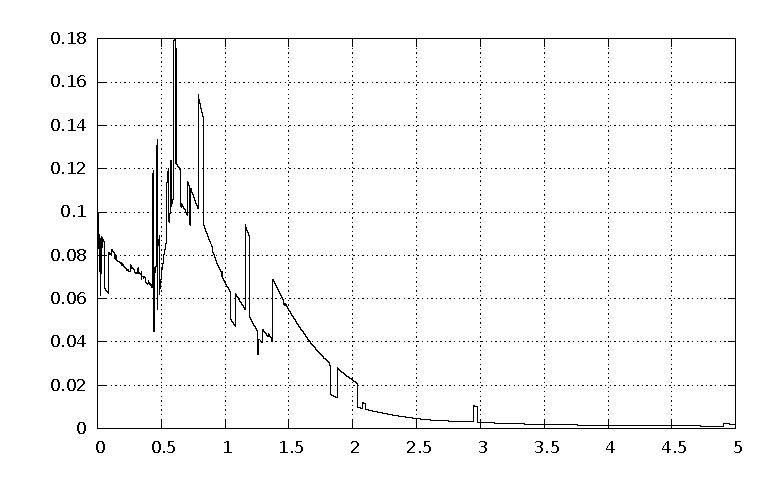
\includegraphics[width=.45\textwidth]
  {figures/nonuniform_bubble_velocity_32_both.ps}
  \caption{($\mu=\gamma=1$) $\|\vec U^m\|_{L^\infty(\Omega)}$ evolution of a
non uniform circle formed by 32 vertices with $C_s=1$ and $C_r=3$ for the
P2--P0 element, uniform mesh.}
  \label{fig:nonuniform_bubble_velocity_32_both}
\end{figure}

Instead, in Figure~\ref{fig:nonuniform_bubble_64_coarse_smooth} are shown some
snapshots of the mesh evolution when an adaptive mesh with characteristic length
$c_l=0.25$ for the boundary and 64 points on the interface is used and no
remeshing is performed. In
Figure~\ref{fig:nonuniform_bubble_velocity_64_coarse_smooth} is shown the
evolution of $\|\vec U^m\|_{L^\infty(\Omega)}$. Also in this case, the
approximations $\Gamma^m$ converge towards an equidistributed circle, while
$\vec U^m$ converges to zero.
\begin{figure}[htbp]
  \centering
  \subfloat[$t=0$]{\includegraphics[width=.45\textwidth]
  {figures/nonuniform_bubble_64_coarse_smooth_000.ps}}\\
  \subfloat[$t=0.5$]{\includegraphics[width=.45\textwidth]
  {figures/nonuniform_bubble_64_coarse_smooth_050.ps}}\quad
  \subfloat[$t=1$]{\includegraphics[width=.45\textwidth]
  {figures/nonuniform_bubble_64_coarse_smooth_100.ps}}\\
  \subfloat[$t=2.5$]{\includegraphics[width=.45\textwidth]
  {figures/nonuniform_bubble_64_coarse_smooth_250.ps}}\quad
  \subfloat[$t=5$]{\includegraphics[width=.45\textwidth]
  {figures/nonuniform_bubble_64_coarse_smooth_500.ps}}\\
  \caption{($\mu=\gamma=1$) Mesh evolution of a non uniform circle formed by
32 vertices with $C_s=1$ and no remeshing for the P2--P0 element, adaptive
mesh.}
  \label{fig:nonuniform_bubble_64_coarse_smooth}
\end{figure}

\begin{figure}[htbp]
  \centering
  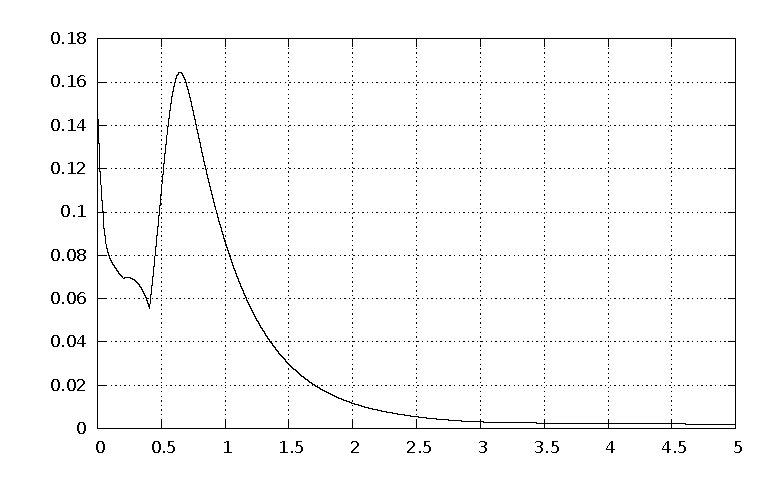
\includegraphics[width=.45\textwidth]
  {figures/nonuniform_bubble_velocity_64_coarse_smooth.ps}
  \caption{($\mu=\gamma=1$) $\|\vec U^m\|_{L^\infty(\Omega)}$ evolution of a
non uniform circle formed by 32 vertices with $C_s=1$ and no remeshing for the
P2--P0 element, adaptive mesh.}
  \label{fig:nonuniform_bubble_velocity_64_coarse_smooth}
\end{figure}

In Figure~\ref{fig:ellipse_both} is reported the pressure evolution of an
ellipse, of axis 0.8 and 0.375, with initial characteristic length $c_l=0.1$,
smoothing coefficient $C_s=1$ and remeshing coefficient $C_r=3$ for the P2--P0
element. We fix the usual domain $\Omega = (-1,1)^2$ and we use the parameters
$\mu=1$, $\gamma=1$, $\tau=10^{-2}$ and $T=10$. The mesh is uniform and we
prescribe homogeneous Dirichlet boundary condition.
Figure~\ref{fig:ellipse_both_volumes} shows the evolution of the bulk inner
relative volume
$\frac{\mathcal{L}^d(\Omega^h_-(t))}{\mathcal{L}^d(\Omega^h_-(0))}$ and the
evolution of the interface length $\mathcal{H}^{d-1}(\Gamma^h(t))$. We point out
that, since there is no exact solution to the problem, we cannot show the
pressure state at $t=0$ therefore we show the pressure state at $t=10^{-5}$.
\begin{figure}[htbp]
  \centering
  \subfloat[$t=10^{-5}$]{\includegraphics[width=.45\textwidth]
  {figures/ellipse_both_000.ps}}\\
  \subfloat[$t=2.5$]{\includegraphics[width=.45\textwidth]
  {figures/ellipse_both_250.ps}}\quad
  \subfloat[$t=5$]{\includegraphics[width=.45\textwidth]
  {figures/ellipse_both_500.ps}}\\
  \subfloat[$t=7.5$]{\includegraphics[width=.45\textwidth]
  {figures/ellipse_both_750.ps}}\quad
  \subfloat[$t=10$]{\includegraphics[width=.45\textwidth]
  {figures/ellipse_both_1000.ps}}\\
  \caption{($\mu=\gamma=1$) Pressure evolution of an ellipse with $c_l=0.1$,
$C_s=1$ and $C_r=3$ for the P2--P0 element, uniform mesh.}
  \label{fig:ellipse_both}
\end{figure}

\begin{figure}[htbp]
  \centering
  \subfloat[$\frac{\mathcal{L}^d(\Omega^h_-(t))}{\mathcal{L}^d(\Omega^h_-(0))}$]
  {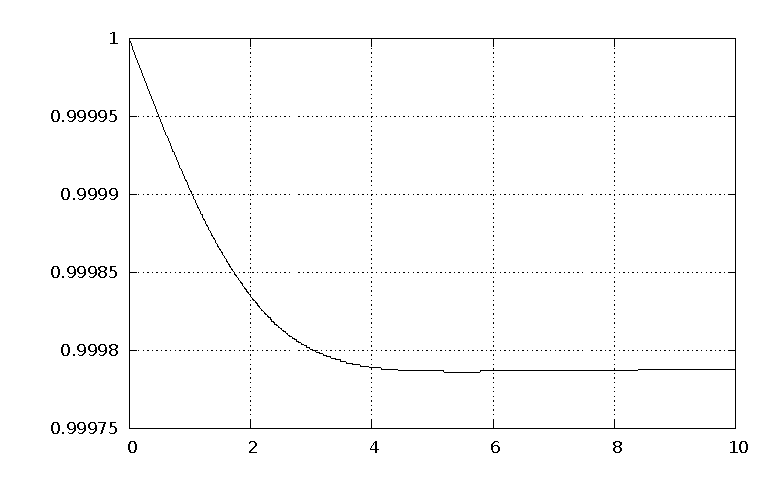
\includegraphics[width=.45\textwidth]
  {figures/ellipse_both_bulk_inner_volume.ps }}
  \subfloat[$\mathcal{H}^{d-1}(\Gamma^h(t))$]
  {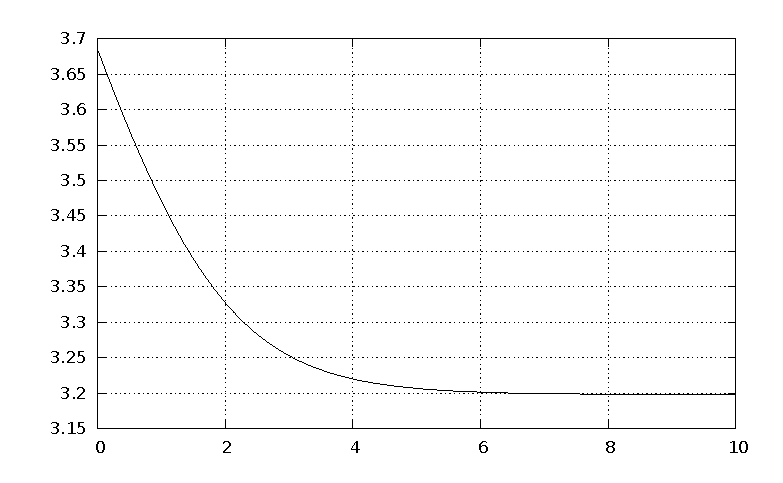
\includegraphics[width=.45\textwidth]
  {figures/ellipse_both_interface_length.ps}}
  \caption{($\mu=\gamma=1$) Bulk inner relative volume evolution and interface
length evolution of an ellipse with $c_l=0.1$, $C_s=1$ and $C_r=3$ for the
P2--P0 element, uniform mesh.}
  \label{fig:ellipse_both_volumes}
\end{figure}

Instead, in Figure~\ref{fig:ellipse_smooth} only the smoothing is used while
the evolution of the bulk inner relative volume and the evolution of the
interface length are shown in Figure~\ref{fig:ellipse_smooth_volumes}.
\begin{figure}[htbp]
  \centering
  \subfloat[$t=10^{-5}$]{\includegraphics[width=.45\textwidth]
  {figures/ellipse_smooth_000.ps}}\\
  \subfloat[$t=2.5$]{\includegraphics[width=.45\textwidth]
  {figures/ellipse_smooth_250.ps}}\quad
  \subfloat[$t=5$]{\includegraphics[width=.45\textwidth]
  {figures/ellipse_smooth_500.ps}}\\
  \subfloat[$t=7.5$]{\includegraphics[width=.45\textwidth]
  {figures/ellipse_smooth_750.ps}}\quad
  \subfloat[$t=10$]{\includegraphics[width=.45\textwidth]
  {figures/ellipse_smooth_1000.ps}}\\
  \caption{($\mu=\gamma=1$) Pressure evolution of an ellipse with $c_l=0.1$,
$C_s=1$ and no remeshing for the P2--P0 element, uniform mesh.}
  \label{fig:ellipse_smooth}
\end{figure}

\begin{figure}[htbp]
  \centering
  \subfloat[$\frac{\mathcal{L}^d(\Omega^h_-(t))}{\mathcal{L}^d(\Omega^h_-(0))}$]
  {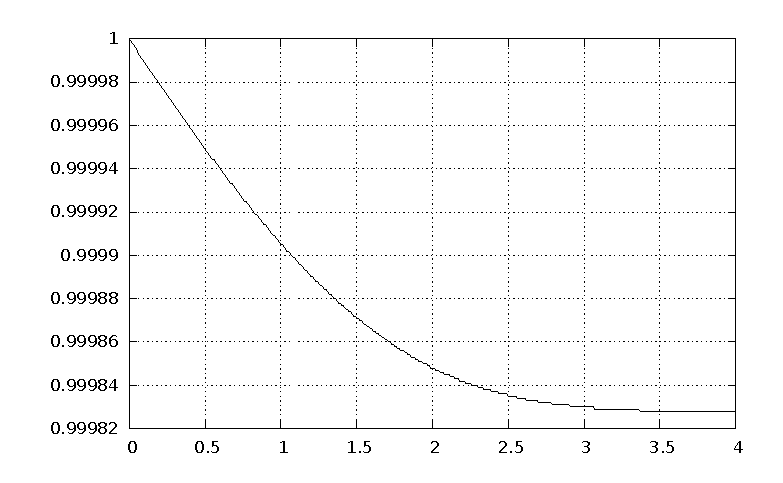
\includegraphics[width=.45\textwidth]
  {figures/ellipse_smooth_bulk_inner_volume.ps}}
  \subfloat[$\mathcal{H}^{d-1}(\Gamma^h(t))$]
  {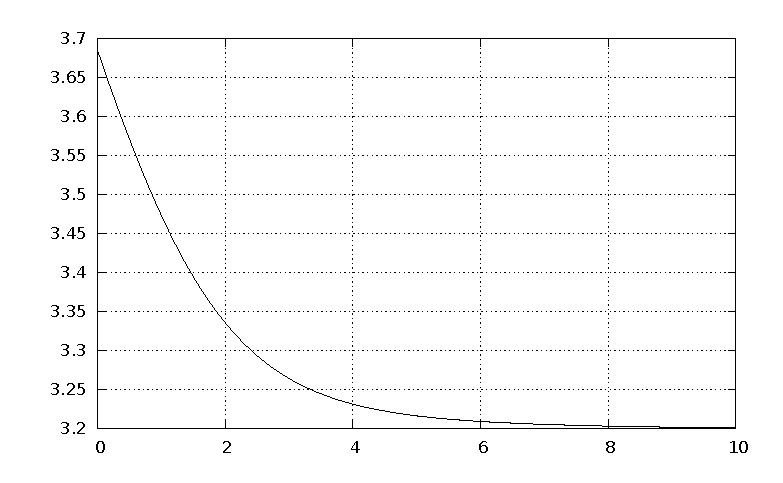
\includegraphics[width=.45\textwidth]
  {figures/ellipse_smooth_interface_length.ps}}
  \caption{($\mu=\gamma=1$) Bulk inner relative volume evolution and interface
length evolution of an ellipse with $c_l=0.1$, $C_s=1$ and no remeshing for the
P2--P0 element, uniform mesh.}
  \label{fig:ellipse_smooth_volumes}
\end{figure}

For the expanding bubble test, we fix $\Omega = (-1,1)^2 \setminus
[-\frac13,\frac13]^2$ and we choose the parameters
\begin{equation*}
\mu_+ = 10\,\mu_- = \gamma = 1,\alpha = 0.15
\end{equation*}
for the true solution (\ref{eq:radialr2},b). In
Figure~\ref{fig:expanding_bubble_uniform} is reported the pressure evolution for
the expanding bubble problem with initial characteristic length $c_l=0.1$,
smoothing coefficient $C_s=1$ and remeshing coefficient $C_r=3$ using an uniform
mesh for the P2--P0 element.
\begin{figure}[htbp]
  \centering
  \subfloat[$t=0$]{\includegraphics[width=.45\textwidth]
  {figures/expanding_bubble_uniform_000.ps}}\\
  \subfloat[$t=0.25$]{\includegraphics[width=.45\textwidth]
  {figures/expanding_bubble_uniform_025.ps}}\quad
  \subfloat[$t=0.5$]{\includegraphics[width=.45\textwidth]
  {figures/expanding_bubble_uniform_050.ps}}\\
  \subfloat[$t=0.75$]{\includegraphics[width=.45\textwidth]
  {figures/expanding_bubble_uniform_075.ps}}\quad
  \subfloat[$t=1$]{\includegraphics[width=.45\textwidth]
  {figures/expanding_bubble_uniform_100.ps}}\\
 \caption{($\mu_+ = 10\,\mu_- = \gamma = 1,\alpha = 0.15$) Pressure evolution
of the 2D expanding bubble with $c_l=0.1$, $C_s=1$ and $C_r=3$ for the P2--P0
element, uniform mesh.}
  \label{fig:expanding_bubble_uniform}
\end{figure}

In Table~\ref{tab:expandingbubble2Delements} it is reported the characteristic
length $c_l$ used to create the initial mesh for the expanding bubble problem,
the corresponding number of interface elements $K_\Gamma$ generated, the
corresponding number of bulk elements $K_\Omega$ generated and the time step
$\tau$ used.
\begin{table*}
 \center
\begin{tabular}{llll}
\hline
$c_l$ & $K_\Gamma$ & $K_\Omega$ & $\tau$\\
\hline
0.25 & 16 & 212 & $1.6\cdot10^{-2}$ \\
0.1 & 32 & 988 & $4\cdot10^{-3}$ \\
0.05 & 64 & 3776 & $10^{-3}$ \\
\hline
\end{tabular}
\caption{Number of interface elements ($K_\Gamma$), number of bulk elements
($K_\Omega$) and time step ($\tau$) for a certain characteristic length ($c_l$)
for the 2D expanding bubble problem, uniform mesh.}
\label{tab:expandingbubble2Delements}
\end{table*}

Some errors for our approximation are shown in
Table~\ref{tab:expandingbubble2Dp2p0remesh} for what concern P2--P0 and in
Table~\ref{tab:expandingbubble2Dp2p1p0remesh} for what concern P2--(P1+P0)  when
a remeshing is performed at each time step and no smoothing is used.
\begin{table*}
 \center
\begin{tabular}{llHllHll}
\hline
$c_l$ & $\errorXx$ & $\LerrorUu2$ & $\errorUu2$ & $\LerrorPp$ & $\errorPp0$ &
$CPU[s]$ & $K_\Omega^T$\\
\hline
0.25 & 5.92892e-03 & 5.38254e-04 & 3.86458e-03 & 4.43308e-01 & 1.52251e-01 &
243 & 120\\
0.1 & 1.46653e-03 & 1.05799e-04 & 8.73181e-04 & 2.14625e-01 & 3.68834e-02 &
4362 & 452\\
0.05 & 3.65445e-04 & 1.48682e-05 & 1.92670e-04 & 8.09743e-02 & 9.20480e-03 &
78947 & 1864\\
\hline
\end{tabular}
\caption{($\mu_+ = 10\,\mu_- = \gamma = 1,\alpha = 0.15$) Expanding bubble
problem on $(-1,1)^2\setminus[-\frac{1}{3},\frac{1}{3}]^2$ over the time
interval $[0,1]$ for the P2--P0 element, with remeshing at every time step and
uniform mesh.}
\label{tab:expandingbubble2Dp2p0remesh}
\end{table*}

\begin{table*}
 \center
\begin{tabular}{llHllHll}
\hline
$c_l$ & $\errorXx$ & $\LerrorUu2$ & $\errorUu2$ & $\LerrorPp$ & $\errorPp1$ &
$CPU[s]$ & $K_\Omega^T$\\
\hline
0.25 & 4.28814e-02 & 2.82404e-02 & 7.79773e-02 & 7.30515e-01 & 1.91554e+00 &
281 & 164\\
0.1 & 2.46288e-02 & 1.14713e-02 & 4.47421e-02 & 5.54819e-01& 1.42510e+00 & 3547
& 464\\
0.05 & 1.24678e-02 & 4.07936e-03 & 2.00263e-02 & 3.97860e-01 & 1.65872e+00 &
68358 & 1880\\
\hline
\end{tabular}
\caption{($\mu_+ = 10\,\mu_- = \gamma = 1,\alpha = 0.15$) Expanding bubble
problem on $(-1,1)^2\setminus[-\frac{1}{3},\frac{1}{3}]^2$ over the time
interval $[0,1]$ for the P2--P1 element, with remeshing at every time step and
uniform mesh.}
\label{tab:expandingbubble2Dp2p1remesh}
\end{table*}

\begin{table*}
 \center
\begin{tabular}{llHllHll}
\hline
$c_l$ & $\errorXx$ & $\LerrorUu2$ & $\errorUu2$ & $\LerrorPp$ &
$\errorPp{1,\rm{DG}}$ & $CPU[s]$ & $K_\Omega^T$\\
\hline
0.25 & 5.95691e-03 & 9.03377e-04 & 4.04415e-03 & 4.44634e-01 & 1.88805e-01 &
258 & 120\\
0.1 & 1.47266e-03 & 2.41766e-04 & 3.23973e-03 & 2.14906e-01 & 4.04825e-02 &
4683 & 452\\
0.05 & 3.65596e-04 & 2.33296e-05 & 2.72450e-04 & 8.10807e-02 & 1.07651e-02 &
129910 & 1864\\
\hline
\end{tabular}
\caption{($\mu_+ = 10\,\mu_- = \gamma = 1,\alpha = 0.15$) Expanding bubble
problem on $(-1,1)^2\setminus[-\frac{1}{3},\frac{1}{3}]^2$ over the time
interval $[0,1]$ for the P2--(P1+P0) element, with remeshing at every time step
and uniform mesh.}
\label{tab:expandingbubble2Dp2p1p0remesh}
\end{table*}

Some errors for our approximation are shown in
Table~\ref{tab:expandingbubble2Dp2p0smooth} for what concern P2--P0 and in
Table~\ref{tab:expandingbubble2Dp2p1p0smooth} for what concern P2--(P1+P0) when
a smoothing with coefficient $C_s=1$ is performed at each time step and no
remeshing is used.
\begin{table*}
 \center
\begin{tabular}{llHllHl}
\hline
$c_l$ & $\errorXx$ & $\LerrorUu2$ & $\errorUu2$ & $\LerrorPp$ & $\errorPp0$ &
$CPU[s]$\\
\hline
0.25 & 5.98661e-03 & 8.42552e-04 & 3.67780e-03 & 4.17354e-01 & 1.52251e-01 &
253\\
0.1 & 1.47669e-03 & 3.40092e-04 & 1.68775e-03 & 2.29737e-01 & 3.68834e-02 &
5348\\
0.05 & 3.68788e-04 & 8.66196e-05 & 5.35566e-04 & 1.05960e-01 & 9.20480e-03 &
107430\\
\hline
\end{tabular}
\caption{($\mu_+ = 10\,\mu_- = \gamma = 1,\alpha = 0.15$) Expanding bubble
problem on $(-1,1)^2\setminus[-\frac{1}{3},\frac{1}{3}]^2$ over the time
interval $[0,1]$ for the P2--P0 element, $C_s=1$, no remeshing and uniform
mesh.}
\label{tab:expandingbubble2Dp2p0smooth}
\end{table*}

\begin{table*}
 \center
\begin{tabular}{llHllHl}
\hline
$c_l$ & $\errorXx$ & $\LerrorUu2$ & $\errorUu2$ & $\LerrorPp$ & $\errorPp1$ &
$CPU[s]$ \\
\hline
0.25 & 3.17165e-02 & 1.96280e-02 & 6.90217e-02 & 6.21614e-01 & 1.91554e+00 &
252\\
0.1 & 1.65835e-02 & 7.58775e-03 & 3.81868e-02 & 4.45878e-01 & 1.42510e+00 &
5570\\
0.05 & 8.04774e-03 & 2.73013e-03 & 1.99853e-02 & 3.15601e-01 & 1.29781e+00 &
145370\\
\hline
\end{tabular}
\caption{($\mu_+ = 10\,\mu_- = \gamma = 1,\alpha = 0.15$) Expanding bubble
problem on $(-1,1)^2\setminus[-\frac{1}{3},\frac{1}{3}]^2$ over the time
interval $[0,1]$ for the P2--P1 element, $C_s=1$, no remeshing and uniform
mesh.}
\label{tab:expandingbubble2Dp2p1smooth}
\end{table*}

\begin{table*}
 \center
\begin{tabular}{llHllHl}
\hline
$c_l$ & $\errorXx$ & $\LerrorUu2$ & $\errorUu2$ & $\LerrorPp$ &
$\errorPp{1,\rm{DG}}$ & $CPU[s]$\\
\hline
0.25 & 6.00787e-03 & 1.39012e-03 & 3.84821e-03 & 4.18178e-01 & 1.88805e-01 &
336\\
0.1 & 1.48003e-03 & 4.40735e-04 & 1.65339e-03 & 2.29815e-01 & 4.04825e-02 &
6114\\
0.05 & 3.68547e-04 & 1.08676e-04 & 8.90397e-04 & 1.05980e-01 & 1.07651e-02 &
18470\\
\hline
\end{tabular}
\caption{($\mu_+ = 10\,\mu_- = \gamma = 1,\alpha = 0.15$) Expanding bubble
problem on $(-1,1)^2\setminus[-\frac{1}{3},\frac{1}{3}]^2$ over the time
interval $[0,1]$ for the P2--(P1+P0) element, $C_s=1$, no remeshing and uniform
mesh.}
\label{tab:expandingbubble2Dp2p1p0smooth}
\end{table*}

In order to choose the better remeshing coefficient $C_r$ several experiment
were carried out. Some errors for our approximation are shown in
Table~\ref{tab:expandingbubble2Dp2p0bothdiffcr} with a starting characteristic
length $c_l=0.1$, using P2--P0 polynomials and smoothing coefficient $C_s=1$.
The better result are obtained with $C_r=3$ because it reduces the number of
remeshing compared to $C_r=2$ while keeping the same performance and error
quality. For this reason we are going to use this parameter for the other
simulations.
\begin{table*}
 \center
\begin{tabular}{llHllHll}
\hline
$C_r$ & $\errorXx$ & $\LerrorUu2$ & $\errorUu2$ & $\LerrorPp$ & $\errorPp0$ &
$CPU[s]$ & $K_\Omega^T$\\
\hline
2 & 1.46658e-03 & 1.05801e-04 & 8.73227e-04 & 2.14589e-01 & 3.68834e-02 & 4297
& 452\\
3 & 1.47162e-03 & 1.02085e-04 & 7.19650e-04 & 2.13599e-01 & 3.68834e-02 & 3919
& 468\\
4 & 1.46761e-03 & 1.27330e-04 & 8.55458e-04 & 2.19071e-01 & 3.68834e-02 & 4682
& 504\\
5 & 1.47218e-03 & 1.26419e-04 & 7.20711e-04 & 2.12456e-01 & 3.68834e-02 & 4775&
468\\
\hline
\end{tabular}
\caption{($\mu_+ = 10\,\mu_- = \gamma = 1,\alpha = 0.15$) Expanding bubble
problem on $(-1,1)^2\setminus[-\frac{1}{3},\frac{1}{3}]^2$ over the time
interval $[0,1]$ for the P2--P0 element, $C_s=1$, $c_l=0.1$ and uniform mesh.}
\label{tab:expandingbubble2Dp2p0bothdiffcr}
\end{table*}

Some errors for our approximation are shown in
Table~\ref{tab:expandingbubble2Dp2p0all} for what concern P2--P0 and in
Table~\ref{tab:expandingbubble2Dp2p1p0all} for what concern P2--(P1+P0) whit
remeshing coefficient $C_r=3$ and with smoothing coefficient $C_s=1$.
\begin{table*}
 \center
\begin{tabular}{llHllHll}
\hline
$c_l$ & $\errorXx$ & $\LerrorUu2$ & $\errorUu2$ & $\LerrorPp$ & $\errorPp0$ &
$CPU[s]$ & $K_\Omega^T$\\
\hline
0.25 & 5.94696e-03 & 6.21713e-04 & 3.34287e-03 & 4.44516e-01 & 1.52251e-01 &
266 & 184\\
0.1 & 1.47162e-03 & 1.02085e-04 & 7.19650e-04 & 2.13599e-01 & 3.68834e-02 &
3919 & 468\\
0.05 & 3.65449e-04 & 1.50098e-05 & 1.74918e-04 & 8.19570e-02 & 9.20480e-03 &
80437 & 1864\\
\hline
\end{tabular}
\caption{($\mu_+ = 10\,\mu_- = \gamma = 1,\alpha = 0.15$) Expanding bubble
problem on $(-1,1)^2\setminus[-\frac{1}{3},\frac{1}{3}]^2$ over the time
interval $[0,1]$ for the P2--P0 element, $C_s=1$, $C_r=3$ and uniform mesh.}
\label{tab:expandingbubble2Dp2p0all}
\end{table*}

\begin{table*}
 \center
\begin{tabular}{llHllHll}
\hline
$c_l$ & $\errorXx$ & $\LerrorUu2$ & $\errorUu2$ & $\LerrorPp$ & $\errorPp1$ &
$CPU[s]$ & $K_\Omega^T$\\
\hline
0.25 & 4.32024e-02 & 2.75478e-02 & 7.80873e-02 & 7.23573e-01 & 1.91554e+00 &
285 & 184\\
0.1 & 2.25864e-02 & 1.03227e-02 & 4.18018e-02 & 5.30421e-01 & 1.42510e+00 &
4275 & 616\\
0.05 & 1.21391e-02 & 3.94487e-03 & 2.07430e-02 & 3.91917e-01 & 1.65872e+00 &
69723 & 1880\\
\hline
\end{tabular}
\caption{($\mu_+ = 10\,\mu_- = \gamma = 1,\alpha = 0.15$) Expanding bubble
problem on $(-1,1)^2\setminus[-\frac{1}{3},\frac{1}{3}]^2$ over the time
interval $[0,1]$ for the P2--P1 element, $C_s=1$, $C_r=3$ and uniform mesh.}
\label{tab:expandingbubble2Dp2p1all}
\end{table*}

\begin{table*}
 \center
\begin{tabular}{llHllHll}
\hline
$c_l$ & $\errorXx$ & $\LerrorUu2$ & $\errorUu2$ & $\LerrorPp$ &
$\errorPp{1,\rm{DG}}$ & $CPU[s]$ & $K_\Omega^T$\\
\hline
0.25 & 5.97759e-03 & 9.03919e-04 & 3.51227e-03 & 4.45378e-01 & 1.88805e-01 &
342 & 184\\
0.1 & 1.47250e-03 & 2.20834e-04 & 2.85624e-03 & 2.13775e-01 & 4.04825e-02 & 4542
& 468\\
0.05 & 3.65594e-04 & 2.33978e-05 & 2.15500e-04 & 8.15265e-02 & 1.07651e-02 &
101190 & 1864\\
\hline
\end{tabular}
\caption{($\mu_+ = 10\,\mu_- = \gamma = 1,\alpha = 0.15$) Expanding bubble
problem on $(-1,1)^2\setminus[-\frac{1}{3},\frac{1}{3}]^2$ over the time
interval $[0,1]$ for the P2--(P1+P0) element, $C_s=1$, $C_r=3$ and uniform
mesh.}
\label{tab:expandingbubble2Dp2p1p0all}
\end{table*}

In all the previous simulations, the meshes used were uniform therefore the
characteristic length was equal for all the nodes. Moreover they were kept
uniform also after the remeshing. Obviously, with this approach, it is very
expensive to have a large number of interface elements since it leads to a
drastic increase of bulk elements. In the following simulations, instead, we use
adaptive meshes which are fine close to the interface and coarse far from the
interface. In Figure~\ref{fig:expanding_bubble_adaptive} is reported the
pressure evolution for the expanding bubble problem with an adaptive mesh which
has characteristic interface length $c_{l,\Gamma}=0.05$ for the P2--P0 element.
This time no smoothing is performed since we need to remesh at each time step.
\begin{figure}[htbp]
  \centering
  \subfloat[$t=0$]{\includegraphics[width=.45\textwidth]
  {figures/expanding_bubble_adaptive_000.ps}}\\
  \subfloat[$t=0.25$]{\includegraphics[width=.45\textwidth]
  {figures/expanding_bubble_adaptive_025.ps}}\quad
  \subfloat[$t=0.5$]{\includegraphics[width=.45\textwidth]
  {figures/expanding_bubble_adaptive_050.ps}}\\
  \subfloat[$t=0.75$]{\includegraphics[width=.45\textwidth]
  {figures/expanding_bubble_adaptive_075.ps}}\quad
  \subfloat[$t=1$]{\includegraphics[width=.45\textwidth]
  {figures/expanding_bubble_adaptive_100.ps}}\\
  \caption{($\mu_+ = 10\,\mu_- = \gamma = 1,\alpha = 0.15$) Pressure evolution
of the 2D expanding bubble with $c_l=0.1$, with remeshing at every time step
for the P2--P0 element, adaptive mesh.}
  \label{fig:expanding_bubble_adaptive}
\end{figure}

The characteristic length of the bulk elements, $c_{l,\Omega}(\vec{x})$, is
computed as
\begin{equation}\label{eq:adaptive_criteria}
 c_{l,\Omega}(\vec{x})=\min\big\{8c_{l,\Gamma},\textrm{dist}(\vec{x},\Gamma)\big\}
\end{equation}
where $\vec{x}\in\partial\Omega$ is a mesh node. See
Table~\ref{tab:expandingbubble2Delements_adaptive} for the resulting number of
elements.
\begin{table*}
 \center
\begin{tabular}{llll}
\hline
$c_{l,\Gamma}$ & $K_\Gamma$ & $K_\Omega$ & $\tau$ \\
\hline
0.01 & 32 & 584 & $6.4\cdot10^{-2}$ \\
0.05 & 64 & 1020 & $1.6\cdot10^{-2}$ \\
0.025 & 128 & 2506 & $4\cdot10^{-3}$\\
0.0123 & 256 & 7460 & $10^{-3}$\\
\hline
\end{tabular}
\caption{Number of interface elements ($K_\Gamma$), number of bulk elements
($K_\Omega$) and time step ($\tau$) for a certain characteristic length ($c_l$)
for the 2D expanding bubble problem, adaptive mesh.}
\label{tab:expandingbubble2Delements_adaptive}
\end{table*}

Some errors for our approximation are shown in
Table~\ref{tab:expandingbubble2Dp2p0adaptive} for what concern P2--P0 and in
Table~\ref{tab:expandingbubble2Dp2p1p0adaptive} for what concern P2--(P1+P0).
\begin{table*}
 \center
\begin{tabular}{llHllHll}
\hline
$c_l$ & $\errorXx$ & $\LerrorUu2$ & $\errorUu2$ & $\LerrorPp$ & $\errorPp0$ &
$CPU[s]$ & $K_\Omega^T$\\
\hline
0.1 & 3.91426e-03 & 6.42479e-04 & 1.86979e-03 & 5.57560e-01 & 2.77033e-01 & 97
& 234\\
0.05 & 9.96943e-04 & 3.65216e-04 & 1.83143e-03 & 2.94448e-01 & 7.13603e-02 &
590 & 564\\
0.025 & 2.51524e-04 & 2.76858e-04 & 2.63245e-03 & 1.51500e-01 & 1.79215e-02 &
11003 & 1226\\
0.0123 & 6.04565e-05 & 6.96741e-05 & 6.90220e-04 & 6.32413e-02 & 4.59376e-03 &
130320 & 3872\\
\hline
\end{tabular}
\caption{($\mu_+ = 10\,\mu_- = \gamma = 1,\alpha = 0.15$) Expanding bubble
problem on $(-1,1)^2\setminus[-\frac{1}{3},\frac{1}{3}]^2$ over the time
interval $[0,1]$ for the P2--P0 element, with remeshing at every time step and
adaptive mesh.}
\label{tab:expandingbubble2Dp2p0adaptive}
\end{table*}

\begin{table*}
 \center
\begin{tabular}{llHllHll}
\hline
$c_l$ & $\errorXx$ & $\LerrorUu2$ & $\errorUu2$ & $\LerrorPp$ & $\errorPp1$ &
$CPU[s]$ & $K_\Omega^T$\\
\hline
0.1 & 3.60050e-02 & 1.98986e-02 & 5.88889e-02 & 6.11708e-01 & 1.13776e+00 & 111
& 232\\
0.05 & 1.87423e-02 & 7.35174e-03 & 3.16821e-02 & 4.58984e-01 & 9.42897e-01 &
1009 & 542\\
0.025 & 8.50687e-03 & 2.30902e-03 & 1.59789e-02 & 3.15820e-01 & 9.12952e-01 &
11979 & 1228\\
0.0123 & 3.86755e-03 & 7.23035e-04 & 6.87523e-03 & 2.19310e-01 & 1.06766e+00 &
124640 & 3854\\
\hline
\end{tabular}
\caption{($\mu_+ = 10\,\mu_- = \gamma = 1,\alpha = 0.15$) Expanding bubble
problem on $(-1,1)^2\setminus[-\frac{1}{3},\frac{1}{3}]^2$ over the time
interval $[0,1]$ for the P2--P1 element, with remeshing at every time step and
adaptive mesh.}
\label{tab:expandingbubble2Dp2p1adaptive}
\end{table*}

\begin{table*}
 \center
\begin{tabular}{llHllHll}
\hline
$c_l$ & $\errorXx$ & $\LerrorUu2$ & $\errorUu2$ & $\LerrorPp$ &
$\errorPp{1,\rm{DG}}$ & $CPU[s]$ & $K_\Omega^T$\\
\hline
32 & 3.96246e-03 & 1.08853e-03 & 4.52252e-03 & 5.58209e-01 & 2.79362e-01 & 120
& 234\\
64 & 1.03381e-03 & 6.47910e-04 & 3.25607e-03 & 2.94451e-01 & 7.22341e-02 & 782
& 564\\
128 & 2.65666e-04 & 5.06483e-04 & 3.35795e-03 & 1.51376e-01 & 3.99953e-02 &
13140 & 1232\\
256 & 6.38812e-05 & 1.54452e-04 & 1.63939e-03 & 6.33098e-02 & 1.66990e-02 &
140630 & 3866\\
\hline
\end{tabular}
\caption{($\mu_+ = 10\,\mu_- = \gamma = 1,\alpha = 0.15$) Expanding bubble
problem on $(-1,1)^2\setminus[-\frac{1}{3},\frac{1}{3}]^2$ over the time
interval $[0,1]$ for the P2--(P1+P0) element, with remeshing at every time step
and adaptive mesh.}
\label{tab:expandingbubble2Dp2p1p0adaptive}
\end{table*}

Finally, we report a shear flow in the domain $\Omega=(-1,1)^2$, with a circle
of radius $r=0.5$ as initial interface. We prescribe the inhomogeneous Dirichlet
boundary condition
\begin{equation*}
\vec g(\vec z)=(z_2,0)^T\quad \mbox{on }\partial\Omega\,,
\end{equation*}
and we use the parameters $\mu=1$, $\gamma=3$, $\tau=10^{-2}$ and $T=5$. In
Figure~\ref{fig:shear_2d} is reported the pressure evolution using a
characteristic length $c_l=0.05$ and an uniform mesh, smoothing coefficient
$C_s=1$ and remeshing coefficient $C_r=3$ for the P2--P0 element. In
Figure~\ref{fig:shear_2d_velocity} is shown the velocity vector field evolution
while the bulk inner relative volume evolution
$\frac{\mathcal{L}^d(\Omega^h_-(t))}{\mathcal{L}^d(\Omega^h_-(0))}$ is reported
in Figure~\ref{fig:shear_2d_bulk_inner_volume}.
\begin{figure}[htbp]
  \centering
  \subfloat[$t=0.5$]{\includegraphics[width=.45\textwidth]
  {figures/2d_shear_050.ps}}\quad
  \subfloat[$t=1$]{\includegraphics[width=.45\textwidth]
  {figures/2d_shear_100.ps}}\\
  \subfloat[$t=2.5$]{\includegraphics[width=.45\textwidth]
  {figures/2d_shear_250.ps}}\quad
  \subfloat[$t=5$]{\includegraphics[width=.45\textwidth]
  {figures/2d_shear_500.ps}}\\
 \caption{($\mu=1,\gamma=3$) Pressure evolution of the 2D shear flow with
$c_l=0.05$, $C_s=1$ and $C_r=3$ for the P2--P0 element, uniform mesh.}
  \label{fig:shear_2d}
\end{figure}

\begin{figure}[htbp]
  \centering
  \subfloat[$t=0.5$]{\includegraphics[width=.45\textwidth]
  {figures/2d_shear_velocity_050.ps}}\quad
  \subfloat[$t=1$]{\includegraphics[width=.45\textwidth]
  {figures/2d_shear_velocity_100.ps}}\\
  \subfloat[$t=2.5$]{\includegraphics[width=.45\textwidth]
  {figures/2d_shear_velocity_250.ps}}\quad
  \subfloat[$t=5$]{\includegraphics[width=.45\textwidth]
  {figures/2d_shear_velocity_500.ps}}\\
  \caption{($\mu=1,\gamma=3$) Velocity vector field of the 2D shear flow with
$c_l=0.05$, $C_s=1$ and $C_r=3$ for the P2--P0 element, uniform mesh.}
  \label{fig:shear_2d_velocity}
\end{figure}

\begin{figure}[htbp]
  \centering
  \includegraphics[width=.45\textwidth]{figures/2d_shear_bulk_inner_volume.ps}
  \caption{($\mu=\gamma=1$) Bulk inner relative volume evolution of the 2D
shear flow with $c_l=0.05$, $C_s=1$ and $C_r=3$ for the P2--P0 element, uniform
mesh.}
  \label{fig:shear_2d_bulk_inner_volume}
\end{figure}

Instead, in Figure~\ref{fig:shear_2d_smooth} the remeshing coefficient is
$C_r=0$ so only the smoothing is used. The bulk inner relative volume evolution
is reported in Figure~\ref{fig:shear_2d_smooth_bulk_inner_volume}.
\begin{figure}[htbp]
  \centering
  \subfloat[$t=0.5$]{\includegraphics[width=.45\textwidth]
  {figures/2d_shear_smooth_050.ps}}\quad
  \subfloat[$t=1$]{\includegraphics[width=.45\textwidth]
  {figures/2d_shear_smooth_100.ps}}\\
  \subfloat[$t=2.5$]{\includegraphics[width=.45\textwidth]
  {figures/2d_shear_smooth_250.ps}}\quad
  \subfloat[$t=5$]{\includegraphics[width=.45\textwidth]
  {figures/2d_shear_smooth_500.ps}}\\
  \caption{($\mu=1,\gamma=3$) Pressure evolution of the 2D shear flow with
$c_l=0.05$, $C_s=1$ and no remeshing for the P2--P0 element, uniform mesh.}
  \label{fig:shear_2d_smooth}
\end{figure}

\begin{figure}[htbp]
  \centering
  \includegraphics[width=.45\textwidth]
  {figures/2d_shear_smooth_bulk_inner_volume.ps}
  \caption{($\mu=\gamma=1$) Bulk inner relative volume evolution of the 2D
shear flow with $c_l=0.05$, $C_s=1$ and no remeshing for the P2--P0 element,
uniform mesh.}
  \label{fig:shear_2d_smooth_bulk_inner_volume}
\end{figure}

\subsection{Numerical results in 3d} \label{subsec:numerical_results_3d}

For the stationary bubble test we use the domain $\Omega = (-1,1)^3$ and we
choose, for the true solution (\ref{eq:radialr},b), the parameters
\begin{equation*}
\mu = \gamma = 1\,.
\end{equation*}
Therefore, the true solution reduces to $r(t) = \frac{1}{2}$, $\vec u(\cdot, t)
= \vec 0$ and $p(t) = 4\,\charfcn{\Omega_-(0)} - \frac{\pi}{12}$ for all
$t\geq0$.

In Table~\ref{tab:bubble3Delements} it is reported the characteristic length
$c_l$, which prescribes the desired size of the elements, used to create the
mesh for the stationary bubble problem, the corresponding number of interface
elements $K_\Gamma$ generated, the corresponding number of bulk elements
$K_\Omega$ generated and the time step $\tau$ used. The interface mesh is
obtained applying a surface diffusion to a sphere until the surface is
stationary which means until the displacement is 0 up to machine accuracy for
all the nodes. The bulk mesh is uniform.
\begin{table*}
 \center
\begin{tabular}{llll}
\hline
$c_l$ & $K_\Gamma$ & $K_\Omega$ & $\tau$ \\
\hline
0.5 & 32 & 408 & $10^{-2}$ \\
0.25 & 220 & 3590 & $10^{-2}$\\
0.125 & 596 & 20473 & $10^{-2}$\\
\hline
\end{tabular}
\caption{Number of interface elements ($K_\Gamma$), number of bulk elements
($K_\Omega$) and time step ($\tau$) for a certain characteristic length ($c_l$)
for the 3D stationary bubble problem, stationary uniform mesh.}
\label{tab:bubble3Delements}
\end{table*}

Since the solution is stationary, neither smoothing nor remeshing is performed.

Some errors for our numerical scheme can be seen in
Table~\ref{tab:bubble3Dp2p0} for the P2--P0 element and in
Table~\ref{tab:bubble3Dp2p1p0} for the P2--(P1+P0).
\begin{table*}
 \center
\begin{tabular}{llHllHl}
\hline
$c_l$ & $\errorXx$ & $\LerrorUu2$ & $\errorUu2$ & $\LerrorPp$ & $\errorPp0$ &
$CPU[s]$ \\
\hline
0.5 & 2.97986e-02 & 0 & 0 & 1.65555e+00 & 7.43095e-01 & 385\\
0.25 & 5.80971e-03 & 0 & 0 & 7.14269e-01 & 1.06521e-01 & 4699\\
0.125 & 2.42857e-03 & 0 & 0 & 3.58466e-01 & 3.83704e-02 & 51604\\
\hline
\end{tabular}
\caption{($\mu=\gamma=1$) Stationary bubble problem on $(-1,1)^3$ over the time
interval $[0,1]$ for the P2--P0 element, stationary uniform mesh.}
\label{tab:bubble3Dp2p0}
\end{table*}

\begin{table*}
 \center
\begin{tabular}{llHllHl}
\hline
$c_l$ & $\errorXx$ & $\LerrorUu2$ & $\errorUu2$ & $\LerrorPp$ & $\errorPp1$ &
$CPU[s]$ \\
\hline
0.5 & 1.56938e-01 & 6.01956e-02 & 1.12442e-01 & 2.10996e+00 & 8.83403e+00 &
315\\
0.25 & 7.28946e-02 & 3.13992e-02 & 6.81154e-02 & 1.47595e+00 & 3.75404e+00 &
4231\\
596 & 4.04291e-02 & 1.34276e-02 & 4.30474e-02 & 1.09674e+00 & 3.73351e+00 &
51287\\
\hline
\end{tabular}
\caption{($\mu=\gamma=1$) Stationary bubble problem on $(-1,1)^3$ over the time
interval $[0,1]$ for the P2--P1 element, stationary uniform mesh.}
\label{tab:bubble3Dp2p1}
\end{table*}

\begin{table*}
 \center
\begin{tabular}{llHllHl}
\hline
$c_l$ & $\errorXx$ & $\LerrorUu2$ & $\errorUu2$ & $\LerrorPp$ &
$\errorPp{1,\rm{DG}}$ & $CPU[s]$ \\
\hline
0.5 & 2.97986e-02 & 0 & 0 & 1.65749e+00 & 7.44770e-01 & 568\\
0.25 & 5.80971e-03 & 0 & 0 & 7.15353e-01 & 2.91977e-01 & 9174\\
0.125 & 2.42857e-03 & 0 & 0 &  3.59181e-01 & 2.96085e-01 & 121110\\
\hline
\end{tabular}
\caption{($\mu=\gamma=1$) Stationary bubble problem on $(-1,1)^3$ over the time
interval $[0,1]$ for the P2--(P1+P0) element, stationary uniform mesh.}
\label{tab:bubble3Dp2p1p0}
\end{table*}

We see that the radius error in Table~\ref{tab:bubble3Dp2p0} is terrible
compared to the analogous test in 2D. The reason is that in 2D the initial
discrete interface is equidistributed and its radius is exactly 0.5 while in 3D
the mesh is equidistributed but the initial radius has already an error. This
error is exactly the one seen in the table since the displacement is always 0 up
to machine accuracy.

Finally, we report a shear flow in the domain $\Omega=(-1,1)^3$, with a sphere
of radius $r=0.5$ as initial interface. The initial interface mesh is a
non-stationary sphere while the bulk mesh is uniform. We prescribe the
inhomogeneous Dirichlet boundary condition
\begin{equation*}
\vec g(\vec z)=(z_3,0,0)^T\quad \mbox{on }\partial\Omega\,,
\end{equation*}
and we use the parameters $\mu=1$, $\gamma=3$, $\tau=10^{-2}$ and $T=5$. In
Figure~\ref{fig:shear_3d} is reported the interface evolution of the sphere with
initial characteristic length $c_l=0.125$, smoothing coefficient $C_s=1$ and
remeshing coefficient $C_r=3$ for the P2--P0 element. The characteristic length
for the boundary is fixed and not uniform like in the 2D case. In
Figure~\ref{fig:shear_3d_velocity} is shown the velocity vector field evolution
in the plane normal to $(0,1,0)$ and passing through the origin while the bulk
inner relative volume evolution
$\frac{\mathcal{L}^d(\Omega^h_-(t))}{\mathcal{L}^d(\Omega^h_-(0))}$ is reported
in Figure~\ref{fig:shear_3d_bulk_inner_volume}.
\begin{figure}[htbp]
  \centering
  \subfloat[$t=0$]{\includegraphics[width=.45\textwidth]
  {figures/3d_shear_000.ps}}\\
  \subfloat[$t=0.5$]{\includegraphics[width=.45\textwidth]
  {figures/3d_shear_050.ps}}\quad
  \subfloat[$t=1$]{\includegraphics[width=.45\textwidth]
  {figures/3d_shear_100.ps}}\\
  \subfloat[$t=2.5$]{\includegraphics[width=.45\textwidth]
  {figures/3d_shear_250.ps}}\quad
  \subfloat[$t=5$]{\includegraphics[width=.45\textwidth]
  {figures/3d_shear_500.ps}}\\
  \caption{($\mu=1,\gamma=3$) Interface evolution of the 3D shear flow with
$c_l=0.125$, $C_s=1$ and $C_r=3$ for the P2--P0 element, uniform mesh.}
  \label{fig:shear_3d}
\end{figure}

\begin{figure}[htbp]
  \centering
  \subfloat[$t=0.5$]{\includegraphics[width=.45\textwidth]
  {figures/3d_shear_velocity_050.ps}}\quad
  \subfloat[$t=1$]{\includegraphics[width=.45\textwidth]
  {figures/3d_shear_velocity_100.ps}}\\
  \subfloat[$t=2.5$]{\includegraphics[width=.45\textwidth]
  {figures/3d_shear_velocity_250.ps}}\quad
  \subfloat[$t=5$]{\includegraphics[width=.45\textwidth]
  {figures/3d_shear_velocity_500.ps}}\\
  \caption{($\mu=1,\gamma=3$) Velocity vector field in the plane normal to
$(0,1,0)$ and passing through the origin of the 3D shear flow with $c_l=0.125$,
$C_s=1$ and $C_r=3$ for the P2--P0 element, uniform mesh.}
  \label{fig:shear_3d_velocity}
\end{figure}

\begin{figure}[htbp]
  \centering
  \includegraphics[width=.45\textwidth]{figures/3d_shear_bulk_inner_volume.ps}
 \caption{($\mu=\gamma=1$) Bulk inner relative volume evolution of the 3D
shear flow with $c_l=0.125$, $C_s=1$ and $C_r=3$ for the P2--P0 element,
uniform mesh.}
  \label{fig:shear_3d_bulk_inner_volume}
\end{figure}

\section{Conclusion}\label{sec:conclusion}
\textcolor{magenta}{TODO : add comparison reults unfitted scheme scheme stokes
paper}

The P2--P0 element has the same accuracy of the P2--(P1+P0) element but it is
simpler to implement, always satisfies the LBB condition and the resulting
linear system is smaller therefore it is the best choice.

The adaptive mesh works very well for the stationary bubble problem. Indeed,
with a fraction of bulk elements, it reaches the same accuracy of the uniform
mesh. Unfortunately this is not the case for the expanding bubble problem. For
this problem, the uniform mesh is much faster and requires less bulk elements
compared to the adaptive mesh therefore.\footnote{But they have different
$\tau$!}

In the 2D expanding bubble problem, We can observe that the simulations which
use only the smoothing have bigger errors and take more time therefore it is not
feasible to use only the smoothing process. On the other side both only
remeshing and smoothing/remeshing combined achieve almost the same quality and
performance. It is important to notice that the performance are almost the same
for sequential code (our case) but in parallel computation the remeshing is the
real bottleneck therefore it is way better to use the combined
smoothing/remeshing approach.

Both element capture perfectly the jump in the pressure.
\newpage
\bibliographystyle{siam}
\bibliography{../bib/robert_refs,../bib/marco_refs}
\end{document}
